\documentclass[
  bibliography=totoc,     % Literatur im Inhaltsverzeichnis
  captions=tableheading,  % Tabellenüberschriften
  titlepage=firstiscover, % Titelseite ist Deckblatt
]{scrartcl}

% Paket float verbessern
\usepackage{scrhack}

% Warnung, falls nochmal kompiliert werden muss
\usepackage[aux]{rerunfilecheck}

% unverzichtbare Mathe-Befehle
\usepackage{amsmath}
% viele Mathe-Symbole
\usepackage{amssymb}
% Erweiterungen für amsmath
\usepackage{mathtools}

% Fonteinstellungen
\usepackage{fontspec}
% Latin Modern Fonts werden automatisch geladen
% Alternativ:
%\setromanfont{Libertinus Serif}
%\setsansfont{Libertinus Sans}
%\setmonofont{Libertinus Mono}
\recalctypearea % Wenn man andere Schriftarten gesetzt hat,
% sollte man das Seiten-Layout neu berechnen lassen

% deutsche Spracheinstellungen
\usepackage{polyglossia}
\setmainlanguage{german}


\usepackage[
  math-style=ISO,    % ┐
  bold-style=ISO,    % │
  sans-style=italic, % │ ISO-Standard folgen
  nabla=upright,     % │
  partial=upright,   % ┘
  warnings-off={           % ┐
    mathtools-colon,       % │ unnötige Warnungen ausschalten
    mathtools-overbracket, % │
},                       % ┘
]{unicode-math}

% traditionelle Fonts für Mathematik
\setmathfont{Latin Modern Math}
% Alternativ:
%\setmathfont{Libertinus Math}

\setmathfont{XITS Math}[range={scr, bfscr}]
\setmathfont{XITS Math}[range={cal, bfcal}, StylisticSet=1]

% Zahlen und Einheiten
\usepackage[
locale=DE,                   % deutsche Einstellungen
separate-uncertainty=true,   % immer Fehler mit \pm
per-mode=symbol-or-fraction, % / in inline math, fraction in display math
]{siunitx}

% chemische Formeln
\usepackage[
version=4,
math-greek=default, % ┐ mit unicode-math zusammenarbeiten
text-greek=default, % ┘
]{mhchem}

% richtige Anführungszeichen
\usepackage[autostyle]{csquotes}

% schöne Brüche im Text
\usepackage{xfrac}

% Standardplatzierung für Floats einstellen
\usepackage{float}
\floatplacement{figure}{htbp}
\floatplacement{table}{htbp}

% Floats innerhalb einer Section halten
\usepackage[
section, % Floats innerhalb der Section halten
below,   % unterhalb der Section aber auf der selben Seite ist ok
]{placeins}

% Seite drehen für breite Tabellen: landscape Umgebung
\usepackage{pdflscape}

% Captions schöner machen.
\usepackage[
  labelfont=bf,        % Tabelle x: Abbildung y: ist jetzt fett
  font=small,          % Schrift etwas kleiner als Dokument
  width=0.9\textwidth, % maximale Breite einer Caption schmaler
]{caption}
% subfigure, subtable, subref
\usepackage{subcaption}

% Grafiken können eingebunden werden
\usepackage{graphicx}
% größere Variation von Dateinamen möglich
\usepackage{grffile}

% schöne Tabellen
\usepackage{booktabs}

% Verbesserungen am Schriftbild
\usepackage{microtype}

% Literaturverzeichnis
\usepackage[style=alphabetic,]{biblatex}
% Quellendatenbank
\addbibresource{lit.bib}

% Hyperlinks im Dokument
\usepackage[
  unicode,        % Unicode in PDF-Attributen erlauben
  pdfusetitle,    % Titel, Autoren und Datum als PDF-Attribute
  pdfcreator={},  % ┐ PDF-Attribute säubern
  pdfproducer={}, % ┘
]{hyperref}
% erweiterte Bookmarks im PDF
\usepackage{bookmark}

% Trennung von Wörtern mit Strichen
\usepackage[shortcuts]{extdash}

\title{V704: Absorption von Gamma- und Beta-Strahlung}
\author{
  Simon Schulte
  \texorpdfstring{
    \\
    \href{mailto:simon.schulte@udo.edu}{simon.schulte@udo.edu}
  }{}
  \texorpdfstring{\and}{, }
  Tim Sedlaczek
  \texorpdfstring{
    \\
    \href{mailto:tim.sedlaczek@udo.edu}{tim.sedlaczek@udo.edu}
  }{}
}
\publishers{TU Dortmund – Fakultät Physik}

\date{Durchführung: 25.04.2017\\
      Abgabe: 02.05.2017}

\begin{document}

\maketitle
\thispagestyle{empty}
\tableofcontents
\newpage
\setcounter{page}{1}
\section{Zielsetzung}
\label{sec:zielsetzung}
Ziel des Versuches ist die Untersuchung des Absorptionsverhaltens von $\beta$-
und $\gamma$-Strahlung.
\section{Theorie}
\label{sec:theorie}
Bei der Betrachtung der Absorption von $\gamma$- und $\beta$-Strahlung
spielen mehrere Begrifflichkeiten eine Rolle.
Im Bezug auf $\gamma$-Strahlung sind der Wirkungsquerschnitt $\sigma$ und
der Absorptionskoeffizient $\mu$ entscheident.
Bei $\beta$-Strahlung wird das Absorptionsverhalten mit der Reichweite
beschrieben.\\

\noindent
Der Wirkungsquerschnitt beschreibt sozusagen die größe der Angriffsfläche
eines Teilchens, im Absorbermaterial, in welcher es zwischen Strahlung
und Teilchen zu Wechselwirkungen kommt.
Im Idealfall ergibt sich ein exponentielles Absorptionsgesetz:
\begin{equation}
  N \left( D \right) = N_0 e^{-n \sigma D}
  \label{eqn:absorption}
\end{equation}
Es gibt die Anzahl der, nach einer Schichtdicke $D$, noch messbaren Ereignisse
einer Ursprungsmenge von $N_0$ an.
Dabei beschreibt der Exponent ($n \sigma D$) die Warscheinlichkeit, dass
es zur Wechselwirkung zwischen einem Strahlungsteilchen und einem Teilchen
des Materials kommt. $n$ ist die Teilchenkonzentration im Absorbermaterial.
Sie berechnet sich nach
\begin{equation}
  n = \frac{z N_\mathup{A}}{V_\mathup{mol}} = \frac{z N_\mathup{A} \rho}{M}.
  \label{eqn:teilchenkonz}
\end{equation}
$N_\mathup{A}$ ist die Avogadro-Konstante und $z$ die Ordnungszahl.
$V_\mathup{mol}$ ist das Molvolumen, welches den Quotienten aus Dichte
$\rho$ und molarer Masse $M$ darstellt.
\begin{equation}
  \mu = n \cdot \sigma
  \label{eqn:mu_theo}
\end{equation}
wird auch als Absorptionskoeffizient bezeichnet.

\subsection{Entstehung und Wechselwirkung von \texorpdfstring{$\gamma$}{gamma}-Strahlung}
$\gamma$-Strahlung entsteht bei energetischen übergängen von Atomkernen.
Wie die Hüllenelektronen können diese unterschiedliche diskrete Energieniveaus
annehmen. Aus der bei einem Übergang in ein tieferes Niveau abgegebenen Energie
kann sich dann ein Photon/$\gamma$-Quant bilden. $\gamma$-Strahlung besitzt die
gleichen Eigenschaften, wie elektromagnetische Wellen und aufgrund der diskreten
Energieniveaus auch ein scharfes Linienspektrum.
Für $\gamma$-Strahlung spielen hauptsächlich drei Arten von Wechselwirkungen
eine Rolle.

\noindent
Der Photo-Effekt beschreibt die Wechselwirkung zwischen einem $\gamma$-Quant
und einem inneren Hüllenelektron eines Absorberteilchens. Dabei wird die volle
Energie des $\gamma$-Quants bei der Ionisierung des Elektrons verbraucht, welches
anschließend die überschüssige Energie des $\gamma$-Quants in Form von kinetischer
Energie erhält. Die Wahrscheinlichkeit, dass dieser Effekt auftritt ist bei schweren
Materialien am größten.

\noindent
Der Compton-Effekt beschreibt die Wechselwirkung zwischen einem $\gamma$-Quant
und einem freien bzw. schwach gebundenen (äußere Hülle) Elektron.
Dieser Effekt ähnelt einem elastischen Stoß. Die Energie des $\gamma$-Quants wird zu
einem Teil zu kinetischer Energie des Elektrons. Babei erfährt das $\gamma$-Quant
eine Richtungsänderung.
Nach Klein und Nishina berechnet sich der Wirkungsquerschnitt für diesen Effekt
nach:
\begin{equation}
  \sigma_\mathup{com} = 2 \pi r_\mathup{e}^2 \left( \frac{1 + \epsilon}{\epsilon^2} \left[ \frac{2 ( 1 + \epsilon)}{1 + 2 \epsilon}-\frac{1}{\epsilon} \mathup{ln}
  ( 1 + 2 \epsilon) \right] + \frac{1}{2 \epsilon} \mathup{ln} ( 1 + 2 \epsilon) - \frac{1 + 3 \epsilon}{( 1 + 2 \epsilon)^2} \right)
  \label{eqn:sigma_theo}
\end{equation}
mit
\begin{equation}
  \epsilon = \frac{E_\gamma}{m_0 c^2} \;\; (m_0 \text{ist die Ruhemasse des Elektrons})
\end{equation}
und
\begin{equation}
  r_\mathup{e} = \frac{e_0^2}{4 \pi \epsilon_0 m_0 c^2} \;\; (\text{klassischer Elektronenradius}).
\end{equation}

\noindent
Zu dem dritten Effekt, der Paarbildung, kommt es erst dann, wenn die Bedingung
\begin{equation}
  E_\gamma > 2 m_0 c^2
\end{equation}
erfüllt ist. Dann bilden sich im Coulomb-Feld eines Absorberteilchens ein Elektron
und ein Positron. $\sigma_\mathup{p}$ ist dabei proportional zu $z^2$.

\noindent
Für Germanium ($z = 32$) sind in Abbildung \ref{fig:V7041} die Verläufe der einzelnen
Koeffizienten, sowie die Überlagerung, in Abhängigkeit von der Energie des
$\gamma$-Quants dargestellt.

\subsection{Entstehung und Wechselwirkung von \texorpdfstring{$\beta$}{beta}-Strahlung}
$\beta$-Strahlung entsteht beim Zerfall eines instabilen Atomkerns.
Dabei ist zwischen zwei Arten von $\beta$-Zerfällen zu unterscheiden.
Dem $\beta^-$- und dem $\beta^+$-Zerfall.

\noindent
Beim $\beta^-$-Zerfall wird aus einem Neutron ein Proton und es entstehen
ein Elektron ($\beta^-$-Teilchen) und ein Antineutrino.

\noindent
Beim $\beta^+$-Zerfall wird aus einem Proton ein Neutron und es entstehen
ein Positron ($\beta^+$-Teilchen) und ein Neutrino.

\noindent
Da bei diesen Zerfällen nicht nur ein Teilchen entsteht und sich die Energie
kontinuierlich auf beide Teilchen verteilt ergibt sich für $\beta$-Strahlung
ein kontinuierliches Spektrum. Die maximale Energie, die das $\beta$-Teilchen
erhält entspricht dabei der bei der Kernumwandlung freigesetzten Energiemenge.
Wegen der geringen Masse der $\beta$-Teilchen treten viele verschiedene Arten
von Wechselwirkungen auf.

\noindent
Die drei wesentlichen sind dabei die Rutherford-Streuung (elastische Streuung
an Atomkernen), inelastische Streuung an Atomkernen bzw. am Coulomb-Feld des
Kerns, bei der Bremsstrahlung entsteht, und inelastische Streuung an
Hüllenelektronen.

\noindent
Trotz der umfangreichen Wechselwirkungsmöglichkeiten zeigt sich, für dünne Schichten
von Absorbermaterial, ein exponentielles Absorptionsverhalten, wie in \eqref{eqn:absorption}.
Erst bei größeren Schichtdicken, die im Bereich der maximalen Reichweite liegen,
zeigen sich stärkere Abweichungen.
\begin{figure}[htb]
  \centering
  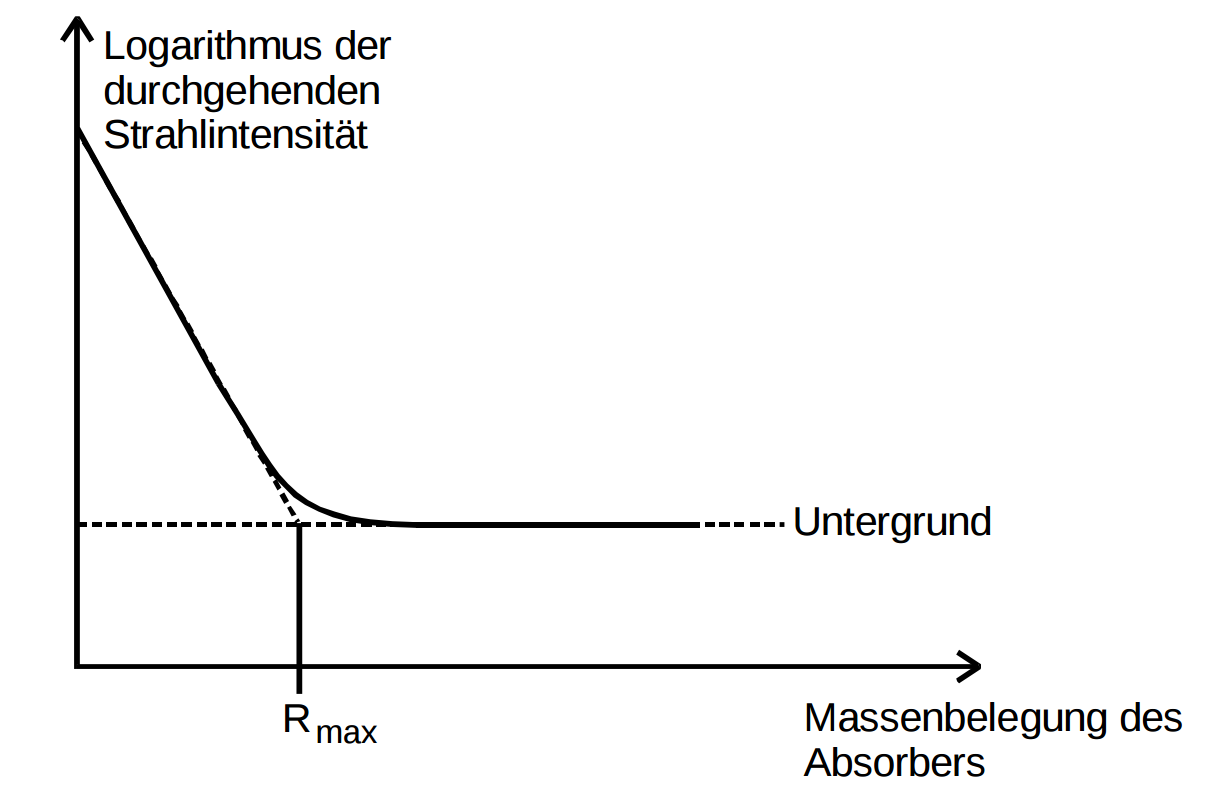
\includegraphics[width=0.9\textwidth]{V7042.png}
  \caption{Absorptionsverhalten eines $\beta$-Strahlers \cite{anleitung}.}
  \label{fig:V7042}
\end{figure}
\begin{figure}[htb]
  \centering
  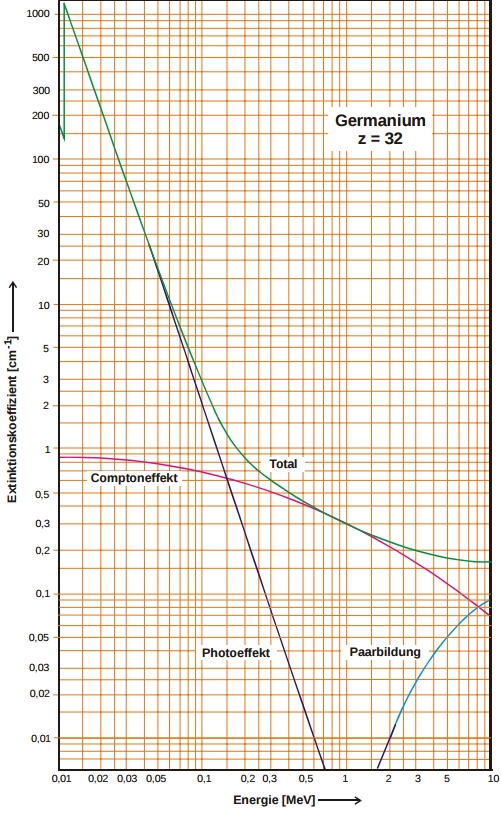
\includegraphics[width=0.9\textwidth]{V7041.png}
  \caption{Absorptionskoeffizienten bei Germanium \cite{anleitung}.}
  \label{fig:V7041}
\end{figure}
In Abbildung \ref{fig:V7042} ist der Verlauf einer Absorptionskurve eines natürlichen
$\beta$-Strahlers dargestellt. Die Strahlungsintensität ist dabei logarithmiert
und in Abhängigkeit von der Massenbelegung dargestellt. Diese Massenbelegung
berechnet sich nach
\begin{equation}
  R = \rho D
  \label{eqn:massenbel}
\end{equation}
und hat die Einheit \si{\gram\per\square\centi\meter}.
Oberhalb der maximalen Reichweite $R_\mathup{max}$ zeigt sich ein Bereich,
in dem eine konstante Intensität gemessen wird. Sie besteht nicht mehr aus
$\beta$-Strahlung, sondern aus anderen durch die Absorption entstandenen
Strahlungs-Effekten, wie der Bremsstrahlung.

\noindent
Über die maximale Reichweite lässt sich auf die maximale Energie der $\beta$-Teilchen
schließen. Dazu wird folgende Formel verwendet:
\begin{equation}
  E_\mathup{max} = \SI{1.92}{\mega\electronvolt\square\centi\meter\per\gram} \sqrt{R_\mathup{max}^2 + \SI{0.22}{\gram\per\square\centi\meter} R_\mathup{max}}
  \label{eqn:E_max}
\end{equation}


\section{Durchführung}
\label{sec:durchführung}
\subsection{Versuchsaufbau}
\begin{figure}[htb]
  \centering
  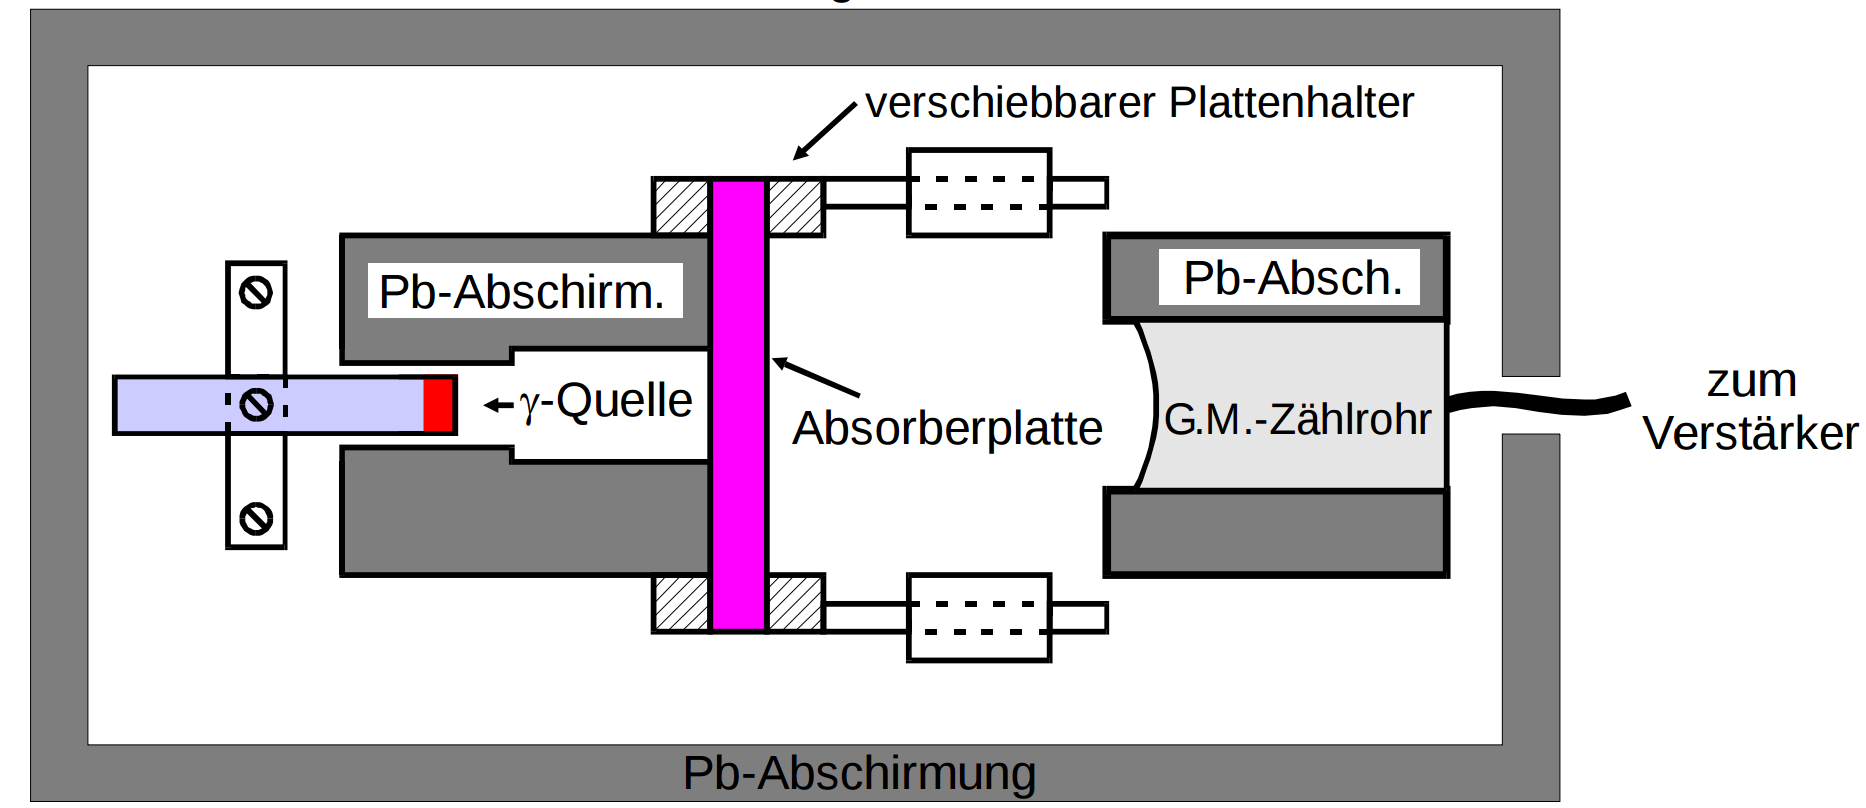
\includegraphics[width=0.9\textwidth]{V7043.png}
  \caption{Schematischer Versuchsaufbau \cite{anleitung}.}
  \label{fig:V7043}
\end{figure}
Bei diesem Versuch wird eine Messapparatur, wie sie in Abbildung \ref{fig:V7043}
zu sehen ist, verwendet. Sie besteht aus einem Geiger-Müller-Zählrohr und einer
Abschirmung aus Blei. Diese dient einerseits dem Strahlenschutz. Andererseits
wird die Messung, auf diese Weise, möglichst frei von äußeren Einflüssen gehalten.
Des Weiteren besitzt die Apparatur eine Halterung für die Probe und eine Halterung
für die Absorberplatten.
\subsection{Versuchsablauf}
Zu Beginn wird eine Nullmessung durchgeführt, bei der, ohne Strahlungsquelle,
die Anzahl an Ereignissen in $\SI{1000}{\second}$ gemessen wird.
Währenddessen sollten die Maße der zur Verfügung stehenden Dämmmaterialien
aufgenommen werden. Anschließend wird eine Quelle an der Apparatur befestigt
und, in zehn Schritten, Dämmmaterial zwischen Quelle und Zählrohr platziert.
Mit jeder Änderung der Dicke des Dämmmaterials wird erneut die Anzahl an
registrierten Ereignissen gemessen. Da die Zählrate mit dicker werdender
Abschirmung immer kleiner wird, muss die Dauer der Messung entsprechend
angepasst werden, um den Fehler der Messungen im Bereich von $\SI{1}{\percent}$
zu halten.
\section{Auswertung}
\label{sec:auswertung}
\subsection{Fehlerrechnung}
\label{sec:fehlerrechnung}
Die in der Auswertung verwendeten Mittelwerte mehrfach gemessener Größen sind gemäß der
Gleichung
\begin{equation}
\bar{x}=\frac{1}{n}\sum_{i=1}^n x_i
\label{eqn:mittelwert}
\end{equation}
bestimmt. Die Standardabweichung des Mittelwertes ergibt sich dabei zu
\begin{equation}
\mathup{\Delta}\bar{x}=\sqrt{\frac{1}{n(n-1)}\sum_{i=1}^n\left(x_i-\bar{x}\right)^2}.
\label{eqn:standardabweichung}
\end{equation}
Resultiert eine Größe über eine Gleichung aus zwei anderen fehlerbehafteten Größen, so
berechnet sich der Gesamtfehler nach der Gaußschen Fehlerfortpflanzung zu
\begin{equation}
\mathup{\Delta}f(x_1,x_2,...,x_n)=\sqrt{\left(\frac{\partial f}{\partial x_1}\mathup{\Delta}x_1\right)^2+\left(\frac{\partial f}{\partial x_2}\mathup{\Delta}x_2\right)^2+ \dotsb +\left(\frac{\partial f}{\partial x_n}\mathup{\Delta}x_n\right)^2}.
\label{eqn:fehlerfortpflanzung}
\end{equation}
Alle in der Auswertung angegebenen Größen sind stets auf die erste signifikante Stelle des
Fehlers gerundet. Setzt sich eine Größe über mehrere Schritte aus anderen Größen zusammen,
so wird erst am Ende gerundet, um Fehler zu vermeiden. Zur Auswertung wird das Programm
Python verwendet.
\subsection{Bestimmung des Absorptionskoeffizienten von Zink und Eisen sowie der Größe $N_0$ der verwendeten radioaktiven Strahlungsquelle}

Zunächst wird der Nulleffekt ausgemessen, den das verwendete Zählrohr detektiert.
Bei Abwesenheit einer radioaktiven Strahlungsquelle registriert das Gerät
$\num{1000}$ Zerfälle in $\SI{1000}{\second}$. Daraus ergibt sich ein Korrekturwert von
\begin{equation}
N_{\mathup{u}}=\frac{\text{Zerfälle}}{\text{Zeit}}=\frac{\SI{1000}{}}{\SI{1000}{\second}}\approx\SI{1}{\frac{1}{\second}}
\label{eqn:nulleffekt}
\end{equation}
für die im Versuch gemessenen Strahlungsintensität ohne einen Strahler. Danach
wurde eine Nullmessung durchgeführt mit dem verwendeten Strahler.
Diese ergab einen Wert von
\begin{equation}
N_{\mathup{0}}=\frac{\text{Zerfälle}}{\text{Zeit}}=\frac{\SI{8599}{}}{\SI{60}{\second}}\approx\SI{143}{\frac{1}{\second}}
\label{eqn:nulleffektmitstrahler}
\end{equation}
für die im Versuch gemessene Strahlungsintensität mit einem Strahler.
Es folgt die Untersuchung der Absorption von $\gamma$-Strahlung durch Zink. Dazu
wird ein $\ce{^{137}Cs}$-Strahler verwendet. Die aufgenommenen Messwerte sind in
Tabelle \ref{tab:Zn} aufgeführt. Dabei bezeichnet $D$ die Schichtdicke, $t$ die
Messzeit und $N$ die Anzahl der vom Zählrohr registrierten Zerfälle.

\begin{table}[H]
\centering
\begin{tabular}{S S S}
\toprule
{$D/\si{\centi\meter}$} & {$N/t$} & {$\sqrt{Z}/Z$}\\
\midrule
{$0,2$} & {$7515/60$} & {$0,001$}\\
{$0,4$} & {$9293/85$} & {$0,01$}\\
{$0,6$} & {$11603/110$} & {$0,01$}\\
{$0,8$} & {$12216/135$} & {$0,01$}\\
{$1,0$} & {$13462/160$} & {$0,01$}\\
{$1,2$} & {$13833/185$} & {$0,01$}\\
{$1,4$} & {$14457/210$} & {$0,01$}\\
{$1,6$} & {$14010/235$} & {$0,01$}\\
{$1,8$} & {$14758/260$} & {$0,01$}\\
{$2,0$} & {$14227/285$} & {$0,01$}\\
\bottomrule
\end{tabular}
\caption{Die Dicke der Zn-Absorber $D$ und zugehörige Zählrate $N$ mit relativem Fehler von $N$. Dabei ist $N= Z/t$.}
\label{tab:Zn}
\end{table}
Die lineare Ausgleichsrechnung ergibt die Geradengleichung
\begin{equation}
    y(x) = (\num{-520(12)})\;x+(\num{4.93(1)}).
    \label{eq:geradengleichung_zink}
\end{equation}

Die angegebenen Unsicherheiten resultieren dabei aus den Unsicherheiten der
linearen Ausgleichsrechnung. Dadurch
folgt für die Zinkproben das exponentielle Absorptionsgesetz

\begin{equation}
    N(d) = N_0\mathup{e}^{-{\mu}d} = \SI{143(1)}{\frac{1}{\second}}\,\mathup{e}^{-\SI{520(12)}{\frac{1}{\metre}}d}.
    \label{eq:absorption_zink}
\end{equation}

Damit ergeben sich für Zink

\begin{equation}
    \boxed{\mu = \SI{520(12)}{\frac{1}{\metre}}} \qquad\text{und}\qquad \boxed{N_0 = \SI{143(1)}{\frac{1}{\second}}}
\end{equation}

Der Graph in Abbildung~\ref{fig:plot_zink} zeigt die Größe $N-N_0$
aufgetragen gegen die Absorberschichtdicke $D$ in einem halblogarithmischen
Diagramm.

Die Auswertung der Messreihe mit Eisen statt Zink erfolgt analog.
Tabelle~\ref{tab:Fe} listet die im Versuch aufgenommenen Werte auf. Die lineare
Ausgleichsrechnung ergibt die Geradengleichung

\begin{equation}
    y(x) = (\num{-510(8)})\;x+(\num{4.92(2)}).
    \label{eq:geradengleichung_eisen}
\end{equation}

\newpage

\begin{table}[H]
\centering
\begin{tabular}{S S S}
\toprule
{$D/\si{\centi\meter}$} & {$N-N_0 \cdot {\si{\second}}$} & {$\sqrt{Z}/Z$}\\
\midrule
{$0,5$} & {$6545/60$} & {$0,01$}\\
{$1,0$} & {$7215/85$} & {$0,01$}\\
{$1,5$} & {$6896/110$} & {$0,01$}\\
{$2,0$} & {$6540/135$} & {$0,01$}\\
{$2,5$} & {$5865/160$} & {$0,01$}\\
{$3,0$} & {$5814/195$} & {$0,01$}\\
{$3,5$} & {$5590/230$} & {$0,01$}\\
{$4,0$} & {$4917/270$} & {$0,01$}\\
{$4,5$} & {$5058/340$} & {$0,01$}\\
{$5,0$} & {$5187/420$} & {$0,01$}\\
\bottomrule
\end{tabular}
\caption{Die Dicke der Fe-Absorber $D$ und zugehörige Zählrate $N$ mit relativem Fehler vom $N$. $N= Z/t$.}
\label{tab:Fe}
\end{table}
Das Absorptionsgesetz für die Eisenproben lautet somit

\begin{equation}
    N(d) = N_0\mathup{e}^{-{\mu}d} = \SI{143(1)}{\frac{1}{\second}}\,\mathup{e}^{-\SI{510(8)}{\frac{1}{\metre}}d}.
    \label{eq:absorption_eisen}
\end{equation}

Als Resultat folgt
%
\begin{equation}
    \boxed{\mu = \SI{510(8)}{\frac{1}{\metre}}} \qquad\text{und}\qquad \boxed{N_0 = \SI{143(1)}{\frac{1}{\second}}}
\end{equation}

\begin{figure}[H]
    \centering
    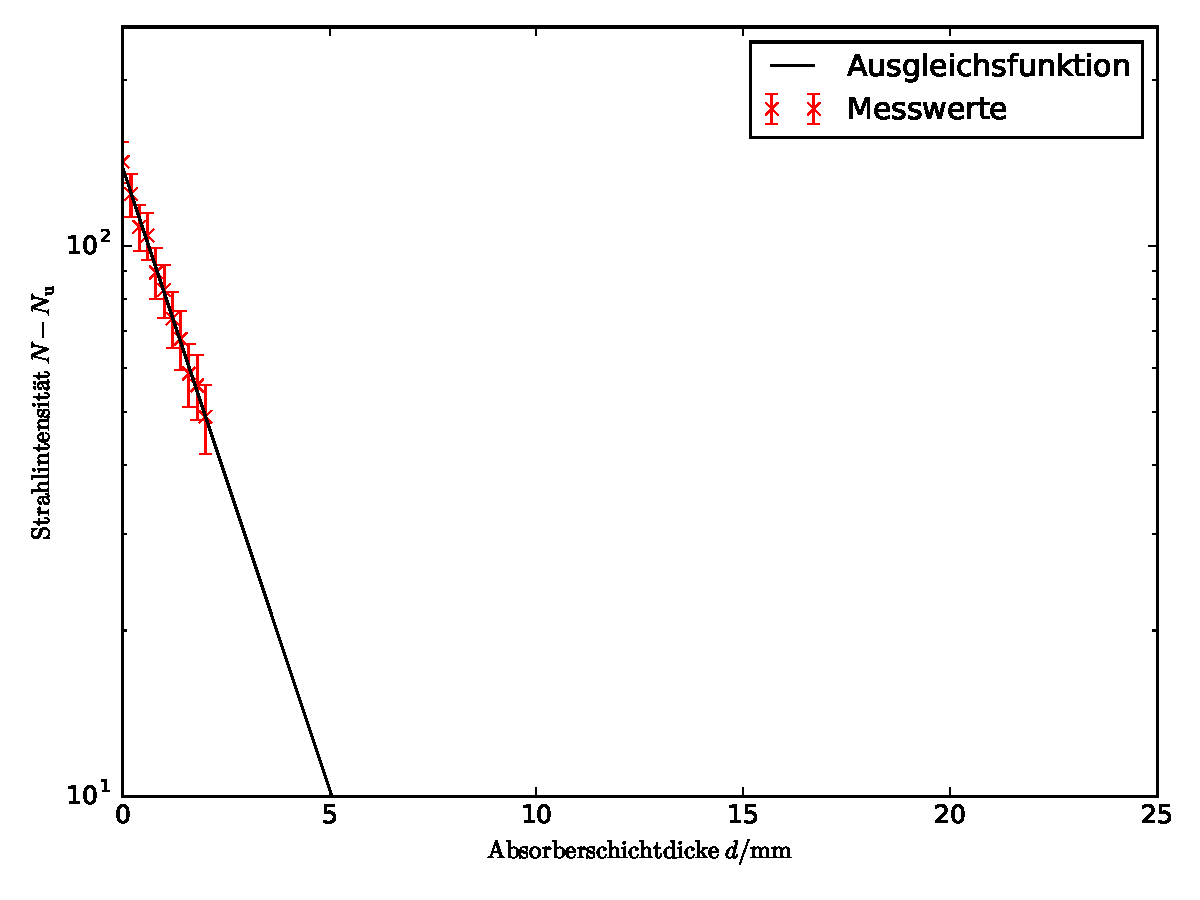
\includegraphics[width=0.80\textwidth]{plot_Zink.pdf}
    \caption{Strahlintensität $N-N_0$ halblogarithmisch aufgetragen gegen die Absorberschichtdicke $D$ von Zink.}
    \label{fig:plot_zink}
\end{figure}

\begin{figure}[H]
    \centering
    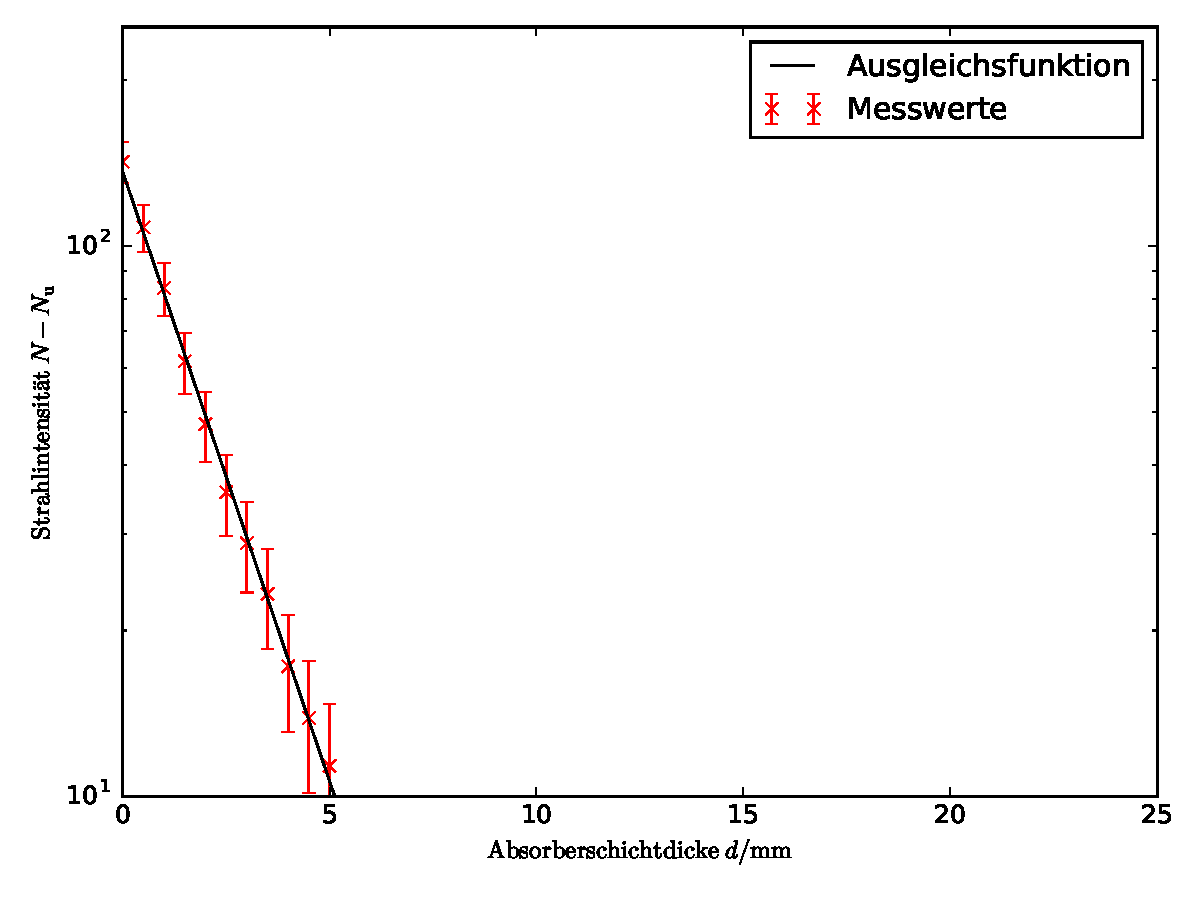
\includegraphics[width=0.80\textwidth]{plot_Eisen.pdf}
    \caption{Strahlintensität ${N-N_0}$ halblogarithmisch aufgetragen gegen die Absorberschichtdicke $D$ von Eisen.}
    \label{fig:plot_eisen}
\end{figure}

\subsection{Vergleich der gemessenen Absorptionskoeffizienten mit den theoretischen Überlegungen}

Um eine Aussage über die im ersten Versuchsteil ablaufenden Absorptionsmechanismen
machen zu können, werden die experimentell bestimmten Absorptionskoeffizienten
mit den theoretisch berechneten Koeffizienten verglichen, die aus Überlegungen
zur Compton-Streuung folgen. Dabei werden die Gleichungen~\eqref{eqn:sigma_theo}
und~\eqref{eqn:mu_theo} aus dem Theorieteil verwendet, wobei für die Berechnung
der Wirkungsquerschnitte $\sigma_{\mathup{com}}$ der für den
$\ce{^{137}Cs}$-Strahler charakteristische Wert $\varepsilon = \num{1.295}$
benutzt wird. Tabelle~\ref{tab:theoriewerte} führt die wesentlichen Größen und
errechneten Werte für Zink und Eisen auf. Dabei bezeichnet $z$ die
Kernladungszahl, $M$ die molare Masse und $\rho$ die Dichte des jeweiligen
Stoffes.

\begin{table}[ht]
	\begin{center}
        \caption{Theoretische Werte für die Absorptionskoeffizienten von Zink und Eisen.}
        \label{tab:theoriewerte}
		\begin{tabular}{l
                        S[table-format = 1.2e-2]
                        S[table-format = 2.0]
                        S[table-format = 3.1]
                        S[table-format = 2.3]
                        S[table-format = 2.2]}
			\toprule
			{Absorber} & {$\sigma_{\mathup{com}}$} & {z} & {$M\left[\si{\frac{\gram}{\mol}}\right]$} &
            {$\rho\left[\si{\frac{\gram}{\centi\metre\cubed}}\right]$} &
            {$\mu_{\mathup{com}}\left[\si{\frac{1}{\metre}}\right]$} \\
			\midrule
			Zink  & 2.57e-29 & 30 &  65.4 &  7.130 & 55 \\
			Eisen & 2.57e-29 & 26 &  55.8 &  7.874 & 62 \\
			\bottomrule
		\end{tabular}
	\end{center}
\end{table}

Es zeigt sich, dass der gemessene Absorptionskoeffizient von Eisen und Zink sehr
stark vom theoretisch ermittelten Wert abweicht. Daraus kann
geschlossen werden, dass zu einem minimalen Teil die Compton-Streuung als
Wechselwirkungsmechanismus zwischen $\gamma$-Quanten und Absorbermaterial
vorliegt. Daraus folgt, dass neben dem Compton-Effekt auch der Photoeffekt einen
gewichtigen Anteil der Wechselwirkungsprozesse ausmachen muss. Die Paarbildung
kann nahezu ausgeschlossen werden, da die Energien der $\gamma$-Quanten
definitiv zu klein sind.

\subsection{Bestimmung der Maximalenergie~\texorpdfstring{$E_{\mathup{max}}$}{R}
eines \texorpdfstring{$\beta$}{β}-Strahlers}

Da für diesen Versuchsteil eine andere Versuchsapparatur verwendet wird, muss
zunächst der Nulleffekt des neuen Zählrohrs bestimmt werden. Bei $\num{327}$
Zerfällen in $\SI{1000}{\second}$ ergibt sich der neue Korrekturwert zu

\begin{equation}
    N_{\mathup{u}}=\frac{\text{Zerfälle}}{\text{Zeit}}=\frac{\SI{327}{}}{\SI{1000}{\second}}\approx\SI{0.33}{\frac{1}{\second}}.
    \label{eq:nulleffekt_2}
\end{equation}^^

Zur Bestimmung der Maximalenergie $E_{\mathup{max}}$ eines $\beta$-Strahlers
wird eine Absorptionskurve für Aluminium aufgenommen. Die Aufnahme der Messwerte
erfolgt wie in den vorangegangenen Versuchsteilen. Als zu untersuchender
Strahler liegt eine $\ce{^{60}Co}$-Probe vor. Tabelle~\ref{tab:beta}
führt die gemessenen Schichtdicken~$D$, die Zeitintervalle~$t$ und die Anzahl der
Zerfälle~$N$ auf. Die Schichtdicken $D$ sind dabei mit Fehlern gegeben.
Diese werden in den weiteren Auswertungsschritten nicht berücksichtigt, da sie
mit unter $\SI{1}{\percent}$ vernachlässigbar klein sind.

\begin{table}[H]
\centering
\begin{tabular}{S S S}
\toprule
{$(D\pm\Delta D)/\si{\micro\meter}$} & {$N/t\si{\per\second}$} & {$\sqrt{N}/N$}\\
\midrule
{$102\pm1$} & {$1772/60$} & {$0,02$}\\
{$126\pm1$} & {$2246/150$} & {$0,02$}\\
{$153\pm0,5$} & {$2296/350$} & {$0,02$}\\
{$160\pm1$} & {$1797/450$} & {$0,02$}\\
{$200\pm1$} & {$847/600$} & {$0,03$}\\
{$253\pm1$} & {$371/700$} & {$0,05$}\\
{$302\pm1$} & {$305/800$} & {$0,06$}\\
{$338\pm5$} & {$401/900$} & {$0,05$}\\
{$400\pm1$} & {$459/1000$} & {$0,05$}\\
\bottomrule
\end{tabular}
\caption{Die Dicke der Absorber $D$ und zugehörige Zählrate $N$ pro Sekunde mit
relativem Fehler vom $N$.}
\label{tab:beta}
\end{table}

Abbildung~\ref{fig:plot_aluminium} zeigt die Strahlungsintensität
aufgetragen gegen die Schichtdicke in einem halblogarithmischen Diagramm. Es ist
deutlich zu erkennen, dass die Kurve zunächst linear abfällt, wie es auch bei
der Absorption von $\gamma$-Strahlung zu beobachten ist. Ab einer Schichtdicke
von circa $d=\SI{250}{\micro\metre}$ bleibt die Strahlungsintensität jedoch
annähernd konstant. Aus den im Theorieteil gemachten Überlegungen kann das
Verhalten wie folgt gedeutet werden: Bei kleinen Schichtdicken zeigt sich ein
ähnliches, exponentielles Absorptionsverhalten der $\beta$-Strahlung, wie bei
der Untersuchung der $\gamma$-Strahlung. Wird die Schichtdicke jedoch zu groß,
überwiegt der Einfluss der Bremsstrahlung, die die $\beta$-Teilchen durch ihre
Ablenkung im Coulomb-Feld der Aluminiumkerne aussenden und die weitaus
durchdringender ist als die geladene ursprüngliche Strahlung.

\begin{figure}[ht]
    \centering
    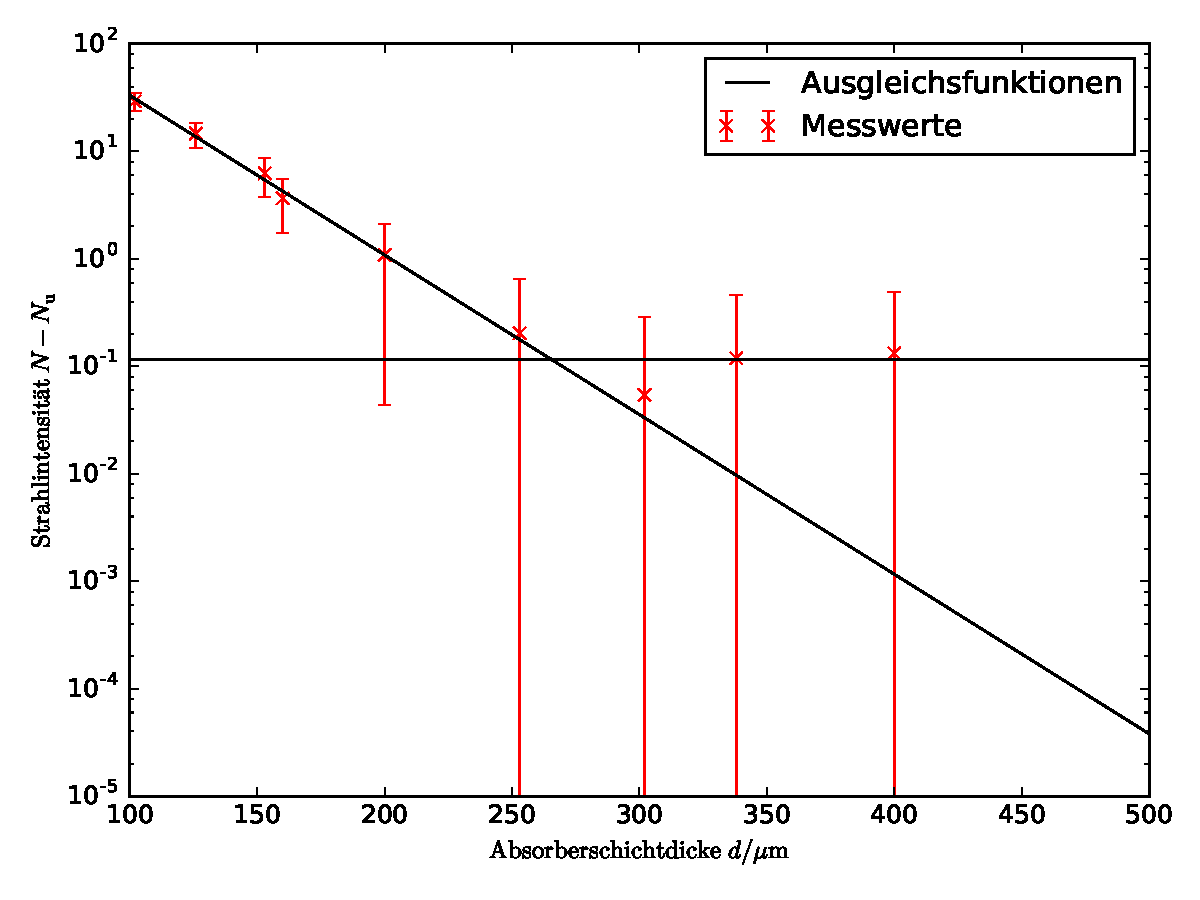
\includegraphics[width=0.80\textwidth]{plot_Aluminium.pdf}
    \caption{Strahlintensität $N-N_0$ halblogarithmisch aufgetragen gegen die Absorberschichtdicke $D$ von Aluminium.}
    \label{fig:plot_aluminium}
\end{figure}

Eine Annäherung des Kurvenverlaufs erfolgt durch die Bestimmmung von zwei
Ausgleichsgeraden. Dabei wird eine Gerade aus den ersten fünf Messpunkten und
die zweite Gerade aus den verbleibenden Messpunkten. Bei der Regression der
zweiten Geraden wird bewusst eine Funktion gesucht, deren Steigung $m_2=0$
beträgt. Der Versuch die Punkte durch eine allgemeine lineare Ausgleichsrechnung
zu approximieren, scheitert insofern, als dass der Wert für die Steigung $m_2$
einen Fehler liefert, der um mehrere Größenordnungen größer ist als der Wert
selbst. Da dies auch im Weiteren viel zu große Fehler verursacht, wird bewusst
eine konstante Funktion gesucht. Es ergeben sich somit die Gleichungen
%
\begin{equation}
    y(x) = m_1\;x+b_1 = (\num{-34000(2000)})\;x+(\num{6.9(3)})
    \label{eq:geradengleichung_aluminium_1}
\end{equation}
%
und
%
\begin{equation}
    y(x) = b_2 = (\num{-2.17(27)}).
    \label{eq:geradengleichung_aluminium_2}
\end{equation}

\newpage

Aus dem Schnittpunkt der Geraden lässt sich die maximale Reichweite
$R_{\mathup{max}}$ der $\beta$-Teilchen im Aluminium durch Ablesen der
$x$-Komponente bestimmen. Der Schnittpunkt ermittelt sich zu

\begin{equation}
    R_{\mathup{max}}=\frac{b_2-b_1}{m_1-m_2}=\SI{27(1)}{\micro\metre},
    \label{eq:reichweite}
\end{equation}

wobei der Fehler gemäß der Gaußschen Fehlerfortpflanzung aus den Fehlern der
Ausgleichsrechnungen resultiert. Da ein fester theoretischer Zusammenhang
zwischen der maximalen Reichweite $R_{\mathup{max}}$ und der Maximalenenergie
$E_{\mathup{max}}$ der $\beta$-Teilchen nur schwer erschlossen werden kann,
wird stattdessen der in Gleichung~\eqref{eqn:E_max} angegebene empirische
Zusammenhang verwendet. Es folgt somit

\begin{equation}
	E_\text{max}=\SI{1,92}{\mega\electronvolt\centi\metre\squared\per\gram}\sqrt{\rho^2\;R_\text{max}^2+\SI{0,22}{\gram\per\centi\metre\squared}\;\rho\;R_\text{max}}=\SI{0.28(5)}{\mega\electronvolt}
\end{equation}

mit der Dichte $\rho = \SI{2.7}{\gram\per\centi\metre\cubed}$ von Aluminium.

\section{Diskussion}
\label{sec:diskussion}
Zusammenfassend listet Tabelle~\ref{tab:ergebnisse} die experimentell
bestimmten Werte auf. Dabei ergibt sich der Wert für $N_m$ aus den beiden
bestimmten Werten im Mittel.

\begin{table}[ht]
	\begin{center}
        \caption{Experimentell bestimmte Werte.}
        \label{tab:ergebnisse}
		\begin{tabular}{lcc}
			\toprule
			& {$\gamma$-Strahlung} & {$\beta$-Strahlung} \\
            & $\ce{^{137}Cs}$ & $\ce{^{60}Co}$ \\
			\midrule
			$\mu_{\text{Zink}}$  & $\SI{520(12)}{\sfrac{1}{\metre}}$   & -                                  \\
            $\mu_{\text{Eisen}}$ & $\SI{510(8)}{\sfrac{1}{\metre}}$    & -                                  \\
            $N_m$                & $\SI{143(1)}{\sfrac{1}{\metre}}$ & -                                  \\
            $R_{\text{max}}$     & -                                  & $\SI{27(1)}{\micro\metre}$         \\
            $E_{\text{max}}$     & -                                  & $\SI{0.28(5)}{\mega\electronvolt}$ \\
			\bottomrule
		\end{tabular}
	\end{center}
\end{table}

Die Fehler der Werte liegen in einem akzeptablen, kleinen Bereich. Daraus folgt,
dass die im Versuch durchgeführte Methodik eine gute Stabilität hat und dass
sich die Ergebnisse leicht reproduzieren lassen. Größte Fehlerquelle des
Versuchs ist der ungewollte Einfluss der natürlichen Strahlung, die niemals
gänzlich abgeschrirmt werden kann und somit immer die Messwerte verfälscht.
Allerdings lässt sich dieser als Nulleffekt genannte Einfluss gut durch eine
präzise Messung bestimmen, sodass die Versuchswerte um diesen Einfluss
korrigiert werden können. Dabei ist der Wert der Korrektur umso besser, je
exakter der Nulleffekt bestimmt wird, dass heißt je länger die natürliche
Strahlung in Abwesenheit der zu untersuchenden radioaktiven Strahlungsquelle
untersucht wird.
\clearpage
\nocite{*}
\printbibliography

\end{document}
